\chapter{Introduction}

\section{What big data are?}

    The term "big data" refers to extremely large and complex datasets that traditional data processing software cannot effectively handle. These datasets are characterized by their volume, velocity, variety, veracity, and value, often referred to as the "5 Vs" of big data.
    There are other definitions that added more V's to the list, like variability, visualization and virality. But we don't care about them.
    The most important thing to know is that big data can create values, in particular:
    \begin{compactitemize}
        \item \textbf{Creating Transparency:} making data accessible to the right stakeholders, in realt ime, can unlock significant value.
        \item \textbf{Enabling Experimentation and performance improvement:} with continuos data collection, organizations can experiment at scale to better understande needs and optimize processes.
        \item \textbf{Segmenting populations for targeted actions:} By analuzing large dataset, companies can identify specific customer segments and tailor prodcuts and services to meet their needs.
        \item \textbf{Enhancing or automating decision-making:} Advanced analytics can support or replace human judgment, reducing risk and uncovering insights that would otherwise go unnoticed.
        \item \textbf{Driving innovation in products, services, and business models:} Big data provides the foundation for creating new offerings, enhancing existing ones, and developing entirely new ways of doing business.
    \end{compactitemize}


\section{The usual pipeline for data analysis}


    The usal pipeline for data analysis is composed by the following steps:
    \begin{compactitemize}
        \item \textbf{Data Generation:} Big data reflected underlying real-word process (eg. from sensor, simulation, experiments,etc.). This raw data is often too large to store entirely and use in its original form.
                                         So gather data in a suitable and efficient way is the first step to make a good analysis.
        \item \textbf{Extraction/Cleaning/Annotation:} Often, the data collected is not immediately suitable for analysis, as it must be extracted from raw sources and transformed into a structured format. This process is technically challenging, requiring precise methods to define and optimize extraction tasks. 
                                                        Morover, data sources, are frequently unreliable: sensor may fail, humand can be biased, and website may be outdated. Recognizing and modelling such errors is essential for developing effective data cleaning techniques, also knows as data \textbf{conditioning},\textbf{massaging} or \textbf{wrangling}.
        \item \textbf{Data Integration, aggregation, and representation:} Effective large-scale analysis relies on collecting heterogeneous data from many sources. Transformation and integration tools help resolve structural and semantic differences, but full integration is often too costly. With the vast availability of data online and the use of integration and analysis tools, new derived data can be produced, raising the challenge of tracking its provenance.
        \item \textbf{Modelling and Analysis:} Methods for querying and mining Big Data differ from traditional statistical analysis on small samples. Big Data is typically noisy, dynamic, heterogeneous, interrelated, and often untrustworthy.
        \item \textbf{Interpretation:} A decision-maker must interpret analytical results by examining assumptions and retracing the analysis. Errors may arise from bugs, model limitations, or flawed data. Systems should allow users to interpret outcomes and repeat analyses with different assumptions or datasets. Ultimately, interpretation often leads to opinions, which may conflict or be weakly supported by the data.
    \end{compactitemize}


\begin{figure}[H]
    \centering
    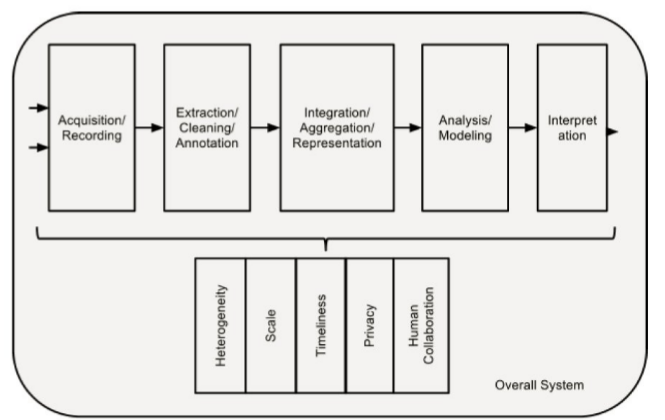
\includegraphics[width=0.6\textwidth]{images/big_data_pipeline.png}
    \caption{Big Data Pipeline}
    \label{fig:Big Data Pipeline}
\end{figure}

\section{Dealing with Big Data}
\subsection{Heterogeneity}

Humans can tolerate messy, heterogeneous data, but data analytics cannot. Algorithms need structured, homogeneous inputs to work reliably. A key challenge is generating metadata that accurately describes the data, known as \textbf{data provenance}, which tracks where data comes from and how it was processed. Provenance is essential, as a single processing error can invalidate downstream results. It allows tracing dependencies and isolating the impact of errors.


\subsection{Inconsistency and Incompleteness}

Big Data originates from diverse and often unreliable sources, so uncertainty, errors, and missing values are common. The scale and redundancy of Big Data help fill missing values, cross-check conflicts, validate patterns, and discover hidden relationships. Even after correction, some errors remain, so analysis must be robust. Managing uncertainty during analysis is a major technical challenge.


\subsection{Data Quality}

Data can be missing or incongruous. Analysts must decide whether to ignore missing values or try to infer them. Incongruities may be errors or may reveal interesting insights. Often, obtaining better or more complete data is impossible, so analysts must work effectively with imperfect data. When data involves human language, challenges grow due to ambiguity and multiple meanings, sometimes requiring LLMs. When automated approaches fail, human intelligence, via crowdsourcing platforms like Amazon Mechanical Turk, can assist with interpretation and annotation.


\subsection{Working with Data at Scale}

Managing vast volumes of data has long been challenging. Traditional relational databases lose effectiveness at large scale, as they prioritize strict consistency for complex transactions, which is often unnecessary for data analysis. Many analyses are comparative rather than absolute, so approximate values are usually sufficient. This led to the rise of NoSQL databases, distributed across many nodes, offering eventual consistency and flexible schemas. Examples include Cassandra, MongoDB, and HBase. Storing data is only part of the challenge; large datasets also require effective processing, often using distributed computing approaches like MapReduce. Machine learning and deep learning are essential tools for analyzing large datasets. Popular libraries include TensorFlow, PyTorch, Scikit-Learn, XGBoost, LightGBM, Hugging Face Transformers, and Spark MLlib. Traditional statistical modeling remains a foundation for data analysis.


\subsection{Machine Learning and Timeliness}

A key challenge is providing interactive, real-time responses to complex queries on high-volume event streams, such as flagging fraudulent transactions. This requires new index structures and methods to summarize, filter, and process data efficiently.


\subsection{Privacy, Ownership, and Human Perspective}

Public concern about the misuse of personal data is high, especially when linking multiple data sources. Organizations must balance leveraging their data for strategic advantage with protecting privacy and controlling sharing. From the human perspective, Big Data analysis must account for human cognitive limits. Visualization and human-in-the-loop approaches help users absorb insights without being overwhelmed. Visual analytics enables understanding and interpretation, as a picture can convey more than a sea of numbers.


\section{Data Science}
\subsection{What is Data Science?}

Data science is the study of data to extract meaningful insights. It is multidisciplinary, combining math, statistics, AI, computer engineering, programming, and storytelling to analyze large datasets and support business decisions. Not all data-driven applications qualify as data science; for example, a typical e-commerce app with a database is data-driven but not data science.


\subsection{Data Science Examples}

CDDB transformed music into a data problem by creating a database of track lengths and album metadata, enabling applications like iTunes to generate value from data rather than audio. Google builds data products such as search spell-checking and tracking epidemics (e.g., Google Flu Trends) by leveraging user behavior and external inputs. Similarly, companies like Facebook, LinkedIn, Instagram, and Amazon use user activity and “data exhaust” to generate recommendations and insights, often combining multiple data sources.

